\chapter{Bleach} \label{cap:metodologia}

\begin{displayquote}
    \begin{center}
        \textit{``Bullet, Claw, Battle Flag, Short Sword. With my fingers bent, I wait for you.''}
    \end{center}
\end{displayquote}

\begin{flushright}
   \textit{-- TITE KUBO}
\end{flushright}

\section{Introduction}
This chapter is dedicated to provide a detailed explanation about the Bleach programming language. Firstly, a brief overview of Bleach's features will be presented by showcasing a few programs written in the language. Then, a detailed breakdown of each of its components and features will be shown to the reader. Afterwards, the challenges encountered during the development of this project will be presented, as well as decisions and trade-offs made. Finally, a comparison between Bleach and the previous languages introduced will be made, as well as a discussion about how Bleach can be properly used to its fullest in an undergraduate Compilers course.

\section{Bleach Overview}
As previously mentioned, this section is dedicated to showcase a few of Bleach's features through the exposition of simple, yet useful, programs to the reader. It's expected that the reader has some familiarity programming with another languages, such as C \cite{kernighan1988c}, C++ \cite{strousrup2000c++}, JavaScript \cite{javascript_language}, Lox \cite{nystrom2021crafting}, Python \cite{python_language} and Ruby \cite{ruby_language}, so the similarities between Bleach and these languages make themselves more evident. \newline

\begin{figure}
    \centering
    \begin{lstlisting}
function greet(){
  print "Hello, World!";
}

greet(); // "Hello, World!"
    \end{lstlisting}
    \caption{Bleach's simplest program: The famous "Hello, World!" program.}
\end{figure}

\begin{figure}
    \centering
    \begin{lstlisting}
function factorial(n){
  if(n == 0){
    return 1;
  }else{
    return n * factorial(n - 1);
  }
}

print factorial(5); // 120
    \end{lstlisting}
    \caption{A Bleach program that shows the usage of recursive functions, if-else statements and arithmetic operators to calculate the factorial of a number.}
\end{figure}

\begin{figure}
    \centering
    \begin{lstlisting}
function main(){
  let numbersInfo = [];
  for(let i = 0; i <= 10; i = i + 1){
    if(i % 2 == 0){
      numbersInfo.append(i + " is even!");
    }else{
      numbersInfo.append(i + " is odd!");
    }
  }
  print numbersInfo;
}

main();
    \end{lstlisting}
    \caption{A Bleach program that shows the usage of for loops and the native \texttt{list} type in order to build a list that contains some information about numbers from 0 to 10.}
\end{figure}

\begin{figure}
    \centering
    \begin{lstlisting}
function quadraticEquationSolver(a, b, c){
  let delta = std::math::pow(b, 2) - 4 * a * c;
  let x1 = (-b + std::math::sqrt(delta))/(2 * a);
  let x2 = (-b - std::math::sqrt(delta))/(2 * a);

  return [x1, x2];
}

print quadraticEquationSolver(1, 0, -4); // [2, -2]
    \end{lstlisting}
    \caption{A Bleach that uses a function which receives the coefficients of a quadratic equation to compute its roots.}
\end{figure}

\begin{figure}
    \centering
    \begin{lstlisting}
class Shape{ // Base Class
  method init(name){
    self.name = name;
  }

  method str() {
    return "This is a " + self.name + ".";
  }

  method area(){ // To be overridden by subclasses
    return 0;
  }
}

class Circle inherits Shape{ // Derived Class
  method init(radius){
    super.init("Circle"); // Call the Base Class constructor
    self.radius = radius;
  }

  method area(){
    return std::math::pow(self.radius, 2) * 3.14159;
  }
}

class Triangle inherits Shape{ // Derived Class
  method init(base, height) {
    super.init("Triangle"); // Call the Base Class constructor
    self.base = base;
    self.height = height;
  }

  method area(){
    return (self.base * self.height) / 2;
  }
}

let c = Circle(5);
let t = Triangle(3, 7);

// This is a Circle. It has an area of 78.539749999999998 units.
print c + " It has an area of " + c.area() + " units.";
// This is a Triangle. It has an area of 10.5 units.
print t + " It has an area of " + t.area() + " units.";
    \end{lstlisting}
    \caption{A Bleach program that illustrates its Object-Oriented features, such as: classes, instances, attributes, methods, overriding and inheritance.}
\end{figure}

\begin{figure}
    \centering
    \begin{lstlisting}
function writeToFile(){
  let userInput = std::io::readLine();
  std::io::fileWrite("output.txt", "w", userInput, true);

  userInput = std::io::readLine();
  std::io::fileWrite("output.txt", "a", userInput, false);

  return;
}

writeToFile();
    \end{lstlisting}
    \caption{A Bleach program that shows its capability with dealing with user-input and writing to \texttt{.txt} files.}
\end{figure}

\section{Bleach Features}
\subsection{Introduction}
This section, as its name suggests, is dedicated to provide to the reader a more extensive and exhausting walkthrough the features available in Bleach. 

\subsection{Data Types}
Bleach has 5 built-in data types made available to the user. Such types are divided into scalar types  and compound types.

Scalar types are types that can represent a single value. In Bleach, there are 3 scalar data types: \texttt{bool}, \texttt{nil} and \texttt{num}.
\begin{itemize}
    \item \texttt{bool}: This data type is used to represent one of two possible values: \texttt{true} or \texttt{false}. Such values are used to express logical conditions and to control the execution of certain parts of a program's source code.
    
    In this context, it's important to mention that Bleach takes inspiration from Ruby and other modern programming languages and implements the concept of "truthy" and "falsey" values in order to evaluate the truthiness or the falseness of values when they are being evaluated inside \texttt{if} statements, loops (\texttt{while}, \texttt{do-while}, \texttt{for}) and ternary operators (\texttt{? :}).

    Essentially, this means that, in Bleach, values of any type (built-in or user-defined) can be used in places where a value of type \texttt{bool} is expected. Moreover, Bleach opted to follow the same convention of Ruby in this matter, which says:

    \begin{itemize}
        \item \textbf{"Falsey" values:} \texttt{false}, \texttt{nil}.
        \item \textbf{"Truthy" values:} Any other value that is not \texttt{false} nor \texttt{nil}.
    \end{itemize}
    
    \item \texttt{nil}: This one is an old acquaintance for most programmers. The \texttt{nil} type has just one possible value: the \texttt{nil} value. In short this value conveys the idea of "no value" or the idea of "absence of a value".

    In other programming languages, this concept appears in other forms, like: \texttt{NULL}, \texttt{nullptr}, \texttt{null}, \texttt{None}, \texttt{nil}, and others. Since Bleach has some influence from Ruby, it adopted \texttt{nil}.
    
    \item \texttt{num}: In favor of simplicity, Bleach has only one type to represent numbers: the \texttt{num} type. This type can be used to represent both integers and floating-point numbers.

    Behind the scenes, the \texttt{num} type is implemented with a double-precision floating-point type, which allows Bleach to cover a lot of territory when it comes to numerical values while still keeping the simplicity initially envisioned for the language.
    
    Finally, with respect to numerical literals, Bleach has support for only basic integer and decimal literals, such as: \texttt{23}, \texttt{42}, \texttt{3.14159}, \texttt{2.71828}, \texttt{-10.4}.
    
\end{itemize}

Compound types are types that can group multiple values into one. In Bleach, there are 2 compound types: \texttt{list} and \texttt{str}.
\begin{itemize}
    \item \texttt{list}: Taking inspiration from Python \cite{python_language}, Bleach has this type. Here, the \texttt{list} type represents an linear-sequence of elements. As previously stated, Bleach is a dynamically-typed language, just like Python. Thus, the \texttt{list} type can store values of different types with no issues. Moreover, Bleach has support for \texttt{list} literals, just as the ones shown below:\newline

    \begin{figure}[H]
        \centering
        \begin{lstlisting}
let l0 = [0, 1, 2, 3, 2.71, 3.14159];
let l1 = ["hello", "there"];
let l2 = [];
let l3 = [false, "Brazil", 9.98, nil];
        \end{lstlisting}
        \caption{Examples of \texttt{list} literals in Bleach.}
    \end{figure}

    Finally, as in Python, the \texttt{list} type in Bleach has the following useful methods that makes the student's life easier when working with this type.
    
    \begin{itemize}
        \item \texttt{append}: Method responsible for adding one value of any type to the end of the \texttt{list} value it was called on. Returns \texttt{nil}.
        \item \texttt{clear}: Method responsible for deleting every element that is currently stored inside the \texttt{list} value it was called on. Returns \texttt{nil}.
        \item \texttt{empty}: Method responsible for checking whether the \texttt{list} value it was called on currently has values stored inside it or not. Returns a \texttt{bool} value.
        \item \texttt{fill}: Method responsible for resizing the \texttt{list} value it was called on to a provided size and also filling all of its indexes with a provided value of any type. Returns \texttt{nil}; 
        \item \texttt{getAt}: Method responsible for returning the value present at the provided index. Returns a value of any type.
        \item \texttt{pop}: Method responsible for deleting and returning the last element present inside a \texttt{list} value, if any. Returns a value of any type.
        \item \texttt{setAt}: Method responsible for setting the value stored at the provided index to the value that was provided. Returns \texttt{nil}.
        \item \texttt{size}: Method responsible for checking and returning the current amount of elements that the \texttt{list} value it was on called on currently has. Return a \texttt{num} value.
    \end{itemize}

    Last but not least, it's important to mention that any misuse of the methods presented above will result in a runtime error during the program's execution.

    \item \texttt{str}: Also taking inspiration from Python \cite{python_language}, Bleach has this type. The \texttt{str} type represents an indexed-sequence of characters (a string), typically used to store and manipulate text. Just as the \texttt{list} type, Bleach also has support for literal values of this type:

    \begin{figure}[H]
        \centering
        \begin{lstlisting}
let s0 = "Ichigo Kurosaki";
let s1 = "Byakuya Kuchiki";
let s2 = "Bazzard Black";
let s3 = "Jugram Haschwalth";
        \end{lstlisting}
        \caption{Examples of \texttt{str} literals in Bleach.}
    \end{figure}

    There are other aspects about the \texttt{str} type that must be mentioned.

    First of all, it is important to recall that it's a sequence type. In short, it means that values of this type can be indexed. In a string, indexing usually allows the programmer to access individual characters from the value, which, in the Bleach programming language, are also values of \texttt{str} type.

    Also, as seen in Figure 4.8, in Bleach, literals values of this type are always enclosed by double quotes (\texttt{""}).

    Finally, as in Python, this type has the following useful methods available:

    \begin{itemize}
        \item \texttt{empty}: Method responsible for checking whether the \texttt{str} value it was called is equal to \texttt{""} or not. Returns a \texttt{bool} value.
        \item \texttt{find}: Method responsible for trying to figure out if the provided sub-string (a \texttt{str} value) exists within the \texttt{str} value the method was called on. Returns a \texttt{num} value which denotes the index at which the sub-string appears, otherwise returns \texttt{-1}. 
        \item \texttt{length}: Method responsible for checking and returning the current amount of characters (which are also values of type \texttt{str}) that the \texttt{str} value it was on called on currently has. Returns a \texttt{num} value.
        \item \texttt{split}: Method responsible for generating a \texttt{list} where each value is of \texttt{str} type. This method receives as its unique argument a value of \texttt{str} type that works as the separator. Returns a \texttt{list} value.
        \item \texttt{substr}: Method responsible for retrieving a sub-string from the \texttt{str} value it was called on. The method receives two arguments of \texttt{num} type that work as the start and end delimiters. Returns a \texttt{str} value.
    \end{itemize}

\end{itemize}

\subsection{Comments}
Even though it is recommendable that a programmer writes code in a way that is readable and understandable, there are certain scenarios where extra explanation about what certain parts of a program's source code is actually doing is necessary.

In these specific cases, programmers usually leave comments in their code that the compiler/interpreter will ignore but people reading their code may find helpful.

Given this, Bleach takes inspiration from C \cite{kernighan1988c} when it comes to support for single-line comments and multi-line comments.

\begin{itemize}
    \item \textbf{Single-Line Comments:} In Bleach, a single-line comment starts with two slashes (\texttt{//}), and the comment continues until the end of the line.
    \item \textbf{Multi-Line Comments:} Bleach also has support for multi-line comments. A multi-line comment has a beginning and an ending. The former is denoted by a (\texttt{/*}), while the later is denoted by a (\texttt{*/}). Everything written in-between is considered a comment and, thus, is ignored by the interpreter at runtime.
\end{itemize}

    \begin{figure}[H]
        \centering
        \begin{lstlisting}
// This is a single-line comment.

/*
This 
is
a
multi-line
comment.
*/
        \end{lstlisting}
        \caption{Examples of \texttt{str} literals in Bleach.}
    \end{figure}

\subsection{Variables}
A variable, as in most programming languages, can be viewed as just a name associated with a storage location in memory. Such storage location is responsible for holding data that can be changed during the execution of a program.

In Bleach this is not different. Variables still have this main functionality. However, they have some particularities that might differ from variables in other programming languages. Such peculiarities are listed below:
\begin{itemize}
    \item In Bleach, all variables are mutable. In other words, once a variable is declared, any amount of assignments are allowed to be performed on this declared variable.
    
    \item A direct consequence of the particularity explained above is that there is no concept of constants in Bleach. There are just mutable variables, as previously mentioned.
    
    \item In Bleach, to declare a new variable, the \texttt{let} keyword must be used:
    \begin{figure}[H]
        \centering
        \begin{lstlisting}
let s = "A value of type 'str'";
        \end{lstlisting}
        \caption{Example of variable declaration in Bleach.}
    \end{figure}
    
    \item In Bleach, if the declaration of a variable does not have an initializer, then, by default, the variable will store the nil value:
    \begin{figure}[H]
        \centering
        \begin{lstlisting}
let someVariable;
print someVariable; // nil
        \end{lstlisting}
        \caption{Example of variable declaration without an initializer in Bleach.}
    \end{figure}

    \item Since Bleach is a dynamically-typed programming language, variables don't have types associated with them. Instead, it's the values stored inside them that have types. The most important consequence of this fact is that a variable can hold a value of different types at different points in time:
    \begin{figure}[H]
        \centering
        \begin{lstlisting}
let a = "hello";
print a; // "hello"

a = nil;
print a; // nil

a = 3.14 + 2.71;
print a // 5.85
        \end{lstlisting}
        \caption{Example demonstrating the fact that, in Bleach, variables do not have types associated.}
    \end{figure}
\end{itemize}

Bleach also has support for global variables, those that have been declared outside of all functions, methods or classes, making them accessible from any part of the program's source code. One point that makes Bleach kind of unique is the fact that the programmer is allowed to re-declare a global variable anytime:
\begin{figure}[H]
    \centering
    \begin{lstlisting}
let pi = 3.14159;
// Write some code in the global scope.
let pi = 9.51413;
    \end{lstlisting}
    \caption{Example demonstrating re-declaration of global variables in Bleach.}
\end{figure}

As expected from most programming language, Bleach supports local variables, which are those declared within a specific block of code, such as a function, method, an \texttt{if-elif-else} statement or a loop statement (\texttt{while}, \texttt{do-while}, \texttt{for}). In this regard, it's important to remember the reader that the scope of a local variable is limited to the block in which it is defined, meaning it can only be accessed and used within that block. Furthermore, once the block of code finishes executing, the local variable is normally destroyed, and its memory is released.
\begin{figure}[H]
    \centering
    \begin{lstlisting}
function foo(){
  let bar = "This is a local variable";
  print bar; // "This is a local variable"

  return;
}

foo();
    \end{lstlisting}
    \caption{Example demonstrating the usage of local variables in Bleach.}
\end{figure}

As previously shown, variables are declared with the usage of the \texttt{let} keyword. Besides, after declaring a variable, the user is allowed to assign different values of different types at different points in time to the declared variable. To do that, the assignment operator (\texttt{=}) comes into play. However, before showing examples of code snippets that make use of this operator, it's very important to mention two semantic details of assignment in Bleach:
\begin{itemize}
    \item In Bleach, an assignment is an expression, not a statement. This means that every assignment produces a value.
    \begin{figure}[H]
        \centering
        \begin{lstlisting}
let foo;
print foo = 20; // 20
        \end{lstlisting}
        \caption{Example showing the behavior of an assignment expression.}
    \end{figure}
    
    \item Bleach allows the user to assign a value to more than one variable in an assignment expression.
    \begin{figure}[H]
        \centering
        \begin{lstlisting}
let x = 20;
let y = 42;

x = y = 13;

print x; // 13;
print y; // 13;
        \end{lstlisting}
        \caption{Example showing the possibility of assigning a value to multiple variable in a single assignment expression.}
    \end{figure}
\end{itemize}

Lastly, the Bleach programming language has support for variable shadowing. In practice, this means that when a variable is declared in an inner scope with the same name of another variable, which was declared in an outer scope, the inner variable "shadows" or hides the variable declared in the outer scope. This means that, until this inner scope ends, every variable reference will "hit" the inner one, not the outer one. In this matter, it is important that in order to create a new scope, the user just needs to use curly braces (\texttt{\{\}}). The two examples presented below show how variable shadowing works in practice in Bleach:
\begin{figure}[H]
    \centering
    \begin{lstlisting}
let a = 42;

print a; // 42

{
  let a = "Hello, there!";
  print a; // "Hello, there!" --> In this scope, the variable a that holds the value "Hello, there!" hides the other one that has the same name but stores a different value: 42.
}

print a; // 42
    \end{lstlisting}
    \caption{First example of variable shadowing in Bleach.}
\end{figure}

\begin{figure}[H]
    \centering
    \begin{lstlisting}
let foo = "hi";
print foo; // "hi"

function f(){
  let foo = 42;
  print foo; // 42;

  return;
}
f();

print foo; // "hi"
    \end{lstlisting}
    \caption{Second example of variable shadowing in Bleach.}
\end{figure}


\subsection{Operators}
Operators in a programming language are tools responsible for executing an operation on one or more operands in order to produce a result.

Operators are fundamental building blocks in every programming language, since they allow data manipulation, computations execution, values comparison, and much more.

This subsection is dedicated to introduce the operators Bleach grants to its users and how each of such operators behave. In the end, an operator precedence table will be shown.

\begin{itemize}
    \item \textbf{Unary Operators:} These operators expects just one operand. Bleach has 2 operators that fall in this class.
        \begin{itemize}
            \item \textbf{Arithmetical:}
                \begin{itemize}
                    \item \textbf{Negation} (\texttt{-}): Negates the value of an operand of type \texttt{num}.
                    \begin{figure}[H]
                        \centering
                        \begin{lstlisting}
let n = 42;
print -n; // -42
                        \end{lstlisting}
                        \caption{Example of usage of the "negation" operator (\texttt{-}).}
                    \end{figure}
                \end{itemize}
            \item \textbf{Logical:}
                \begin{itemize}
                    \item \textbf{Not} (\texttt{!}): Inverts the value of an operand of type \texttt{bool}.
                    \begin{figure}[H]
                        \centering
                        \begin{lstlisting}
let b = true;
print !b; // false
print !!b; // true
                        \end{lstlisting}
                        \caption{Example of usage of the "not" operator (\texttt{!}).}
                    \end{figure}                    
                \end{itemize}
        \end{itemize}
    \item \textbf{Binary Operators:} These operators expects just two operands. Bleach has 13 operators that fall in this class.
        \begin{itemize}
            \item \textbf{Arithmetical:}
                \begin{itemize}
                    \item \textbf{Addition} (\texttt{+}): This operator expects two operands, which can be of type \texttt{num} or \texttt{str}. However, the action performed by this operator at runtime depends on the types of the operands provided.

                    If both operands are values of type \texttt{num}, then this operator adds the first (left) operand to the second (right) operand and returns the result (a value of type \texttt{num}).
                    \begin{figure}[H]
                        \centering
                        \begin{lstlisting}
print 2 + 3; // 5
print 2.71 + 3.14159; // 5.85159
                        \end{lstlisting}
                        \caption{First example of usage of the "addition" operator (\texttt{+}).}
                    \end{figure}

                    If both operands are values of type \texttt{str}, then this operator concatenates the first (left) operand to the second (right) operand and returns the result (a value of type \texttt{str}).
                    \begin{figure}[H]
                        \centering
                        \begin{lstlisting}
print "hello," + " there!"; // "hello, there!"
print "a" + "b"; // "ab"
                        \end{lstlisting}
                        \caption{Second example of usage of the "addition" operator (\texttt{+}).}
                    \end{figure}

                    If one operand is a value of type \texttt{num} and the other one is a value of type \texttt{str}, then the one that is a \texttt{num} is converted into its \texttt{str} representation and concatenated to the other operand. The operator then returns the result (a value of type \texttt{str}).
                    \begin{figure}[H]
                        \centering
                        \begin{lstlisting}
print 2 + "two"; // "2two"
                        \end{lstlisting}
                        \caption{Third example of usage of the "addition" operator (\texttt{+}).}
                    \end{figure}
                    
                    
                    \item \textbf{Subtraction} (\texttt{-}): This operator expects two operands of type \texttt{num}. It subtracts the second (right) operand from the first (left) operand, and returns the result (a value of type \texttt{num}).
                    \begin{figure}[H]
                        \centering
                        \begin{lstlisting}
print 5 - 3; // 2
                        \end{lstlisting}
                        \caption{Example of usage of the "subtraction" operator (\texttt{-}).}
                    \end{figure}
                    
                    \item \textbf{Multiplication} (\texttt{*}): This operator expects two operands of type \texttt{num}. It multiplies the first (left) operand by the second (right) operand, and returns the result (a value of type \texttt{num}).
                    \begin{figure}[H]
                        \centering
                        \begin{lstlisting}
print 1.5 * 4; // 6
                        \end{lstlisting}
                        \caption{Example of usage of the "multiplication" operator (\texttt{*}).}
                    \end{figure}
                    
                    \item \textbf{Division} (\texttt{/}): This operator expects two operands of type \texttt{num}. It divides the first (left) operand, also called dividend, by the second (right) operand, also called divisor, and returns the result of the division (a value of type \texttt{num}). It is worth mentioning that if the value of the divisor is \texttt{0}, then a runtime error will be thrown.
                    \begin{figure}[H]
                        \centering
                        \begin{lstlisting}
print 5 / 2; // 2
print 1 / 3; // 0.333333333333333
                        \end{lstlisting}
                        \caption{Example of usage of the "division" operator (\texttt{/}).}
                    \end{figure}

                    
                    \item \textbf{Remainder} (\texttt{\%}): This operator expects two operands of type \texttt{num}. It divides the first (left) operand, also called dividend, by the second (right) operand, also called divisor, and returns the remainder of this division (a value of type \texttt{num}). It is worth mentioning that if the value of the divisor is \texttt{0}, then a runtime error will be thrown. Moreover, a runtime error will also be thrown if both operands are not integer numbers. If the reader wants to computer the remainder of a division between decimal numbers, then he/she/they should use the  \texttt{std::math::fmod} native function, which is presented at section 4.3.9.
                    \begin{figure}[H]
                        \centering
                        \begin{lstlisting}
print 5 % 2; // 1
print 1 % 3; // 1
print -10 % 4 // -2
                        \end{lstlisting}
                        \caption{Example of usage of the "remainder" operator (\texttt{\%}).}
                    \end{figure}
                
                
                \end{itemize}
                
            \item \textbf{Comparison:}
                \begin{itemize}
                    \item \textbf{Greater Than} (\texttt{>}): This operator expects two operands of type \texttt{num}. It checks if the first (left) operand is greater than the second (right) operand. If that is indeed the case, it returns \texttt{true}. Otherwise, it returns \texttt{false}.
                    \begin{figure}[H]
                        \centering
                        \begin{lstlisting}
print 5 > 2; // true
print 1 > 3; // false
                        \end{lstlisting}
                        \caption{Example of usage of the "greater than" operator (\texttt{>}).}
                    \end{figure}

                    \item \textbf{Greater Than or Equal} (\texttt{>=}): This operator expects two operands of type \texttt{num}. It checks if the first (left) operand is greater than or equal to the second (right) operand. If that is indeed the case, it returns \texttt{true}. Otherwise, it returns \texttt{false}.
                    \begin{figure}[H]
                        \centering
                        \begin{lstlisting}
print 5 >= 2; // true
print -1 >= -1 // true
print 1 >= 3; // false
                        \end{lstlisting}
                        \caption{Example of usage of the "greater than or equal" operator (\texttt{>=}).}
                    \end{figure}

                    \item \textbf{Lesser Than} (\texttt{<}): This operator expects two operands of type \texttt{num}. It checks if the first (left) operand is lesser than the second (right) operand. If that is indeed the case, it returns \texttt{true}. Otherwise, it returns \texttt{false}.
                    \begin{figure}[H]
                        \centering
                        \begin{lstlisting}
print 5 < 2; // false
print 1 < 3; // true
                        \end{lstlisting}
                        \caption{Example of usage of the "lesser than" operator (\texttt{<}).}
                    \end{figure}

                    
                    \item \textbf{Lesser Than or Equal} (\texttt{<=}): This operator expects two operands of type num. It checks if the first (left) operand is lesser than or equal to the second (right) operand. If that is indeed the case, it returns \texttt{true}. Otherwise, it returns \texttt{false}.
                    \begin{figure}[H]
                        \centering
                        \begin{lstlisting}
print 5 <= 2; // false
print 0 <= 0; // true
print 1 <= 3; // true
                        \end{lstlisting}
                        \caption{Example of usage of the "lesser than or equal" operator (\texttt{<=}).}
                    \end{figure}
                \end{itemize}
                
            \item \textbf{Equality:}
                \begin{itemize}
                    \item \textbf{Equal} (\texttt{==}): This operator expects two operands of the following built-in types (\texttt{bool}, \texttt{nil}, \texttt{num}, \texttt{str}). It checks whether the values are of the same type and, if that's the case, checks whether such values are the same. Returns \texttt{true} if both conditions are true. Otherwise, returns \texttt{false}.
                    \begin{figure}[H]
                        \centering
                        \begin{lstlisting}
print 2 == 2; // true
print 2 == (1 + 1); // true
print 2 == 3; // false
print "hello" == "hello"; // true
print "hello" == "hell"; // false
print 2 == nil; // false
print nil == nil; // true
print true == true; // true
print true == false; // false
print true == !!true; // true
                        \end{lstlisting}
                        \caption{Example of usage of the "equal" operator (\texttt{==}).}
                    \end{figure}

                    
                    \item \textbf{Not Equal} (\texttt{!=}): This operator expects two operands of the following built-in types (\texttt{bool}, \texttt{nil}, \texttt{num}, \texttt{str}). It checks whether the values are not of the same type and, if they are of the same type, it then checks whether such values are not the same. Returns \texttt{true} if one (or both) conditions mentioned above are not satisfied. Otherwise, returns \texttt{false}.
                    \begin{figure}[H]
                        \centering
                        \begin{lstlisting}
print 2 != 2; // false
print 2 != (1 + 1); // false
print 2 != 3; // true
print "hello" != "hello"; // false
print "hello" != "hell"; // true
print 2 != nil; // true
print nil != nil; // false
print true != true; // false
print true != false; // true
print true != !!true; // false
                        \end{lstlisting}
                        \caption{Example of usage of the "not equal" operator (\texttt{!=}).}
                    \end{figure}
                \end{itemize}
                
            \item \textbf{Logical:}
                \begin{itemize}
                    \item \textbf{And} (\texttt{and}): This operator returns \texttt{true} if, and only if, both operands are "truthy" values. Otherwise, it returns \texttt{false}. This operator performs short-circuiting whenever possible.
                    \begin{figure}[H]
                        \centering
                        \begin{lstlisting}
print 5 and 2; // true
print 5 and false; // false
print false and nil; // false
                        \end{lstlisting}
                        \caption{Example of usage of the "and" operator (\texttt{and}).}
                    \end{figure}
                    
                    \item \textbf{Or} (\texttt{or}): This operator returns \texttt{true} if one of its operands is a "truthy" value. Otherwise, it returns \texttt{false}. As the operator above, this one also performs short-circuiting whenever possible.
                                        \begin{figure}[H]
                        \centering
                        \begin{lstlisting}
print 5 or 2; // true
print 5 or false; // true
print false or nil; // false
                        \end{lstlisting}
                        \caption{Example of usage of the "or" operator (\texttt{or}).}
                    \end{figure}
                \end{itemize}
        \end{itemize}
    \item \textbf{Ternary Operator:}
        A ternary operator is, as its name suggests, an operator that expects three operands. Bleach has just one operator that falls in this class (\texttt{? :}), the one the reader is probably familiar with from C and C++.
    
        This operator provide another way of executing conditional operations. It is used to evaluate a condition and return one of two values based on whether the condition evaluates to \texttt{true} or \texttt{false}.

        The three operands expected by the ternary operator can be of any type (built-in or user-defined). The first one is evaluated by the ternary operator with respect to its truthiness of falseness. If the value is "truthy", then the operator returns the second operand. Otherwise, it returns the third operand.

        \begin{figure}[H]
            \centering
            \begin{lstlisting}
print 2 == 2 ? "2 is equal to 2" : "2 is not equal to 2"; // "2 is equal to 2"
            \end{lstlisting}
            \caption{Example of usage of the "ternary" operator (\texttt{? :}).}
        \end{figure}

    \item \textbf{Bleach's Operators Precedence Table:}
        \begin{table}[H]
        \centering
        \begin{tabular}{|c|c|}
            \hline
            \textbf{Precedence} & \textbf{Operators} \\  % First row: header
            \hline
            1 & \texttt{!}, \texttt{-} (unary) \\  % Start adding data
            \hline
            2 & \texttt{*}, \texttt{/}, \texttt{\%} \\
            \hline
            3 & \texttt{+}, \texttt{-} (binary) \\
            \hline
            4 & \texttt{>}, \texttt{>=}, \texttt{<}, \texttt{<=} \\
            \hline
            5 & \texttt{==}, \texttt{!=} \\
            \hline
            6 & \texttt{and} \\
            \hline
            7 & \texttt{or} \\
            \hline
            8 & \texttt{? :} \\
            \hline
            9 & \texttt{=} (assignment) \\
            \hline
        \end{tabular}
        \caption{Bleach's Operator Precedence Table.}
        \label{tab:example}
        \end{table}
\end{itemize}

\subsection{Control-Flow Structures}
Control-Flow structures are entities that allow the programmer to dictate in what order and by how many times instructions or code blocks are executed.

These entities are responsible for allowing branching mechanisms, decision-making and repetition in a program. The main consequence of this is that a program can have a more dynamic and sophisticated behavior.

In Bleach, there are 3 classes of control-flow structures:
\begin{itemize}
    \item \textbf{Conditional Statements:} These statements are known to execute a block of code based on the fact that certain condition(s) are satisfied. Bleach has support for \texttt{if} statements, which may be followed by any amount of \texttt{elif} statements and a unique \texttt{else} statement, in this order. Bleach also provides support for nesting \texttt{if} statements, which gives more flexibility to the user.
\begin{figure}[H]
    \centering
    \begin{lstlisting}
let number = 15;

if(number % 3 and number % 5){
  print "Fizz Buzz"; // Executes this statement.
}elif(number % 3){
  print "Fizz";
}elif(number % 5){
  print "Buzz";
}else{
  print number;
}
    \end{lstlisting}
    \caption{First example that shows the usage of \texttt{if}, \texttt{elif} and \texttt{else} in Bleach.}
\end{figure}

\begin{figure}[H]
    \centering
    \begin{lstlisting}
let number = 10;

if(number > 0){
  if(number % 2 == 0){
    // Executes this block of code.
    print "The number " + number + " is positive and even!";
  }else{
    print "The number " + number + " is positive and odd!";
  }
}else{
  print "The number " + number + " is negative!";
}
    \end{lstlisting}
    \caption{Second example that shows the usage of \texttt{if}, \texttt{elif} and \texttt{else} in Bleach.}
\end{figure}

    It is important to mention that the \texttt{if}, \texttt{elif} and \texttt{else} statements require a block after it. Otherwise, a syntax error will be thrown by the interpreter. This happens because such statements create a new local scope.
    
    \item \textbf{Loop statements:} These ones are used to allow the repetition of a code block based on a certain condition. Bleach has support for 3 different types of loop statements: \texttt{while}, \texttt{do-while} and \texttt{for}. Just as in conditional statements, Bleach also allows the nesting of loop statements.
\begin{figure}[H]
    \centering
    \begin{lstlisting}
let counter = 10;

while(counter > 0){
  counter = counter - 1;
}

print counter; // 0
    \end{lstlisting}
    \caption{Example that shows the usage of a \texttt{while} loop in Bleach.}
\end{figure}

\begin{figure}[H]
    \centering
    \begin{lstlisting}
let counter = 1;

do{
  counter = counter - 1;
}while(counter > 1);

print counter; // 0
    \end{lstlisting}
    \caption{Example that shows the usage of a \texttt{do-while} loop in Bleach.}
\end{figure}

\begin{figure}[H]
    \centering
    \begin{lstlisting}
let number;

for(number = 10; number > 0; number = number - 1){}

print number; // 0
    \end{lstlisting}
    \caption{Example that shows the usage of a \texttt{for} loop in Bleach.}
\end{figure}

    It is important to mention that these statements also require a block after them. Otherwise, a syntax error will be thrown by the interpreter. This happens because they also create a new local scope, just as the conditional statements.

    \item \textbf{Jump statements:} Jump statements are used by the programmer to alter the execution flow of the source code by "jumping" to a different part of it. Bleach has support for 3 types of jump statements: \texttt{break}, \texttt{continue} and \texttt{return}.

\begin{figure}[H]
    \centering
    \begin{lstlisting}
let numbers = [];

for(let i = 0; i < 10; i = i + 1){
  if(i == 5){
    break;
  }
  numbers.append(i);
}

print numbers; // [0, 1, 2, 3, 4]
    \end{lstlisting}
    \caption{Example that shows the usage of a \texttt{break} statement in Bleach.}
\end{figure}

\begin{figure}[H]
    \centering
    \begin{lstlisting}
let numbers = [];

for(let i = 0; i <= 10; i = i + 1){
  if(i % 2 == 1){
    continue;
  }
  numbers.append(i);
}

print numbers; // [0, 2, 4, 6, 8, 10]
    \end{lstlisting}
    \caption{Example that shows the usage of a \texttt{continue} statement in Bleach.}
\end{figure}

\begin{figure}[H]
    \centering
    \begin{lstlisting}
function foo(){
  print "alpha";

  return;

  print "omega"; // Not reachable due to the "return" keyword.
}

foo(); // "alpha"
    \end{lstlisting}
    \caption{Example that shows the usage of a \texttt{return} statement in Bleach.}
\end{figure}
\end{itemize}

\subsection{Functions}
\textbf{Falar como ocorre a passagem de valores em chamadas de função: por valor ou por referência.}

Functions, as is widely known, are fundamental building blocks in programming. They are reusable blocks of code created with the intention of executing a specific job. Therefore, they allow programmers to organize, reuse, and manage code in a more organized manner.

Functions can take inputs, process them and also return a value. As mentioned above, they are very useful because they are helpful when it comes down to breaking complex problems into smaller and simpler chores.

The code snippet below shows an example of a function declaration statement in Bleach:

\begin{figure}[H]
    \centering
    \begin{lstlisting}
function functionName(parameter1, parameter2, parameter3){
  // Code to be executed
  return value;
}
    \end{lstlisting}
    \caption{Example of function declaration statement in Bleach.}
\end{figure}

Still regarding function declaration statements, it is relevant to mention that if the programmer omits the \texttt{return} statement from it, then when such function is called at runtime it will, by default, return the \texttt{nil} value.

In Bleach, function calls are no different than in the most famous programming languages. The programmer is expected to call it by its name and provide the necessary arguments, according to its respective declaration statement. The code snippet below shows how to properly call a function in Bleach.

\begin{figure}[H]
    \centering
    \begin{lstlisting}
function subtract(a, b){
  return a + b;
}

let x = 5;
let y = 3;
let answer = subtract(a, b);

print answer; // 2
    \end{lstlisting}
    \caption{Example of a function call in Bleach.}
\end{figure}

As happens in most dynamically-typed programming languages, when a function call does not comply with its respective declaration statement, a runtime error is thrown.

It is very important to mention that functions in Bleach have certain limitations: They don't have support optional parameters, nor for default value for its parameters, and also cannot be overloaded. \textbf{("Future Work" Material? Assignment to students?)}

Going further, in Bleach, functions are first-class values. Basically, this means that a function is not different from any other value in Bleach. This fact implies in the consequences listed below:

\begin{itemize}
    \item Functions can be assigned to variables.
    \item Functions can be passed as arguments to other functions.
    \item Functions can be returned from other functions.
    \item Functions can be stored inside data structures.
\end{itemize}

Finally, Bleach also has support for anonymous functions, also known as lambda functions. As the name suggests, these are functions that do not have a name attached to them (i.e., they are declared without a name). Usually, famous programming languages have syntax mechanisms that permit such a thing. Bleach opted for taking a mixed approach by using the \texttt{lambda} keyword, used in Python, as well as an "arrow" token (\texttt{->}). When it comes to semantics, anonymous functions are just as powerful as the default ones.

The code snippet shown below demonstrates how to use an anonymous function in Bleach:

\begin{figure}[H]
    \centering
    \begin{lstlisting}
    let add = lambda -> (a, b){ return a + b; }
    
    let answer = add(10, 15);
    
    print answer; // 25
    \end{lstlisting}
    \caption{Example of an anonymous function usage in Bleach.}
\end{figure}


\subsection{The Object-Oriented Paradigm in Bleach}
\textbf{(Não sei se essa subseção ficou muito bem escrita. Poderia dar uma olhada com mais atenção nela?)}

As previously stated, Bleach is a multi-paradigm programming language, since it has support both the procedural and the object-oriented paradigms.

When it comes to the object-oriented paradigm, Bleach has support to the following features of it, such as: classes, attributes/fields, methods, instances, the \texttt{self} keyword and inheritance. These features allow the reader to build modular, reusable, and maintainable code by organizing software into objects, entities that are capable of representing both data and behavior.

The rest of this subsection is dedicated to provide a more in-depth overview about each of the mentioned features:

\begin{itemize}
    \item \textbf{Classes:} As is common knowledge among undergraduate CS students, in the object-oriented paradigm, a class is basically a "blueprint" for creating instances/object. Regarding this, since Bleach is a dynamically-typed language, it made sense for it to take the same route as Python: It does not require explicit type information about attributes and methods. Furthermore, there is a lot of flexibility when it comes to additions, because the programmer can add new attributes and methods at runtime to instances of a class, as will be shown later in this subsection. In order to declare a new class, the user must use the \texttt{class} keyword followed by the name of the declared class and curly braces (\texttt{\{\}}):
\begin{figure}[H]
    \centering
    \begin{lstlisting}
// The declaration of a class called "Person".
class Person{
  method init(name, age){
    self.name = name;
    self.age = age;
  }

  method greet(){
    return "I am " + self.name + " and I have " + self.age + " years.";
  }
}
    \end{lstlisting}
    \caption{Example of a class declaration in Bleach.}
\end{figure}

    \item \textbf{Instances/Objects:} When it comes to instances/objects, Bleach took the same approach that was taken by Lox and Python. An instance/object is a concretization of a class. In other words, an instance is an entity created at runtime that has the structure and behavior defined by its class declaration. However, it is important to remember that each instance of a class can store its own unique data. In essence, an instance of a class has its own copy of the class’s attributes, but they share the class's methods.

    Since Bleach took the same approach to deal with instances/objects as Lox, it is safe to say that the following quote written by Robert Nystrom in \cite{nystrom2021crafting} also applies to Bleach: "Instances are loose bags of data and you can freely add fields to them as you see fit using normal imperative code."
    
    \item \textbf{The \texttt{self} keyword:} The keyword \texttt{self} serves for a very specific purpose inside a class: It's a reference to the current instance/object of the class. This keyword allows methods within a class to access the specific instance's attributes and other methods.
    
    In addition to that, the \texttt{self} keyword assists to clarify when local variables (parameters that receive passed arguments in a method call, for example) have the same name as instance variables.

    Finally, this keyword permits methods to return the current instance, which allows method chaining: a scenario where multiple methods can be called in sequence on the same instance.

    The code snippet shown below demonstrates a more sophisticated use of the \texttt{self} keyword:
\begin{figure}[H]
    \centering
    \begin{lstlisting}
class Counter{
  method init(){
    self.count = 0;
  }

  method increment(){
    self.count = self.count + 1;
    return self;
  }
}
let counter = Counter();
counter.increment().increment().increment();
print counter.count; // 3;
    \end{lstlisting}
    \caption{Example of a more refined use of the \texttt{self} keyword in Bleach.}
\end{figure}
    
    \item \textbf{Attributes:} As seen in the item above, attributes don't need to have type annotations attached to them. Instead, the attributes' types are determined when values are assigned to them at runtime. On top of that, attributes of a class can store values of different types at different points in time. As in most programming languages that are object-oriented, in order to access the attributes of a class, one must use the "dot" (\texttt{.}) notation, as displayed below:
\begin{figure}[H]
    \centering
    \begin{lstlisting}
class Square{
  method init(length){
    self.length = length;
  }
}

let square = Square(5);

print square.length; // 5

square.area = square.length * square.length;
print square.area; // 25

square.perimeter = 4 * square.length;
print square.perimeter; // 20
    \end{lstlisting}
    \caption{Example that illustrates the usage of attributes of a class in Bleach.}
\end{figure}

    \textbf{Falar sobre a implicação semântica de ter um método e um atributo com o mesmo nome em uma instância de uma classe.}

    \item \textbf{Methods:} In Bleach, methods of a class don't have type annotations in their signature, just like functions. The types are checked during runtime when the method is called, which can potentially throw a runtime error if a value of an unexpected type is passed as an argument. In order to declare a method of a class in Bleach, the programmer can use the same syntax as in a function declaration, just needing to replace the \texttt{function} keyword by the \texttt{method} keyword. To call a method of a class, it is required to use the "dot" notation (\texttt{.}) combined with the function calling convention (\texttt{()}), as exhibited below:
\begin{figure}[H]
    \centering
    \begin{lstlisting}
class Dog{
  method bark(){
    return "Owf Owf!";
  }
}

let dog = Dog();

print dog.bark(); // "Owf Owf!"
    \end{lstlisting}
    \caption{Example that illustrates the usage of methods of a class in Bleach.}
\end{figure}

    Last but not least, since default functions and anonymous functions are values in Bleach, it is completely possible to add new methods to an instance of a class by using them, as demonstrated below:
\begin{figure}[H]
    \centering
    \begin{lstlisting}
class Dog{
  method bark(){
    return "Owf Owf!";
  }
}

let dog = Dog();

dog.louderBark = lambda -> (){ return "WOOF!"; };
print dog.louderBark(); // "WOOF!"
    \end{lstlisting}
    \caption{Example that illustrates the addition of a new method to an instance of a class during runtime.}
\end{figure}
    
    \textbf{Falar sobre os métodos especiais "init" e "str". Ambos podem ser omitidos na declaração de uma classe. O que acontece quando eles são omitidos? Quais as implicações disso?}

    
    \item \textbf{Inheritance and the \texttt{super} keyword:} In Bleach, as in other popular languages like C++, Java and Python, inheritance allows the user to create a new class based on an existing class, extending or modifying its functionality.

    Bleach follows a very similar implementation of inheritance to that of Python with just one major difference: For simplicity purposes, Bleach only supports single inheritance whereas Python has support for multiple inheritance.

    In order to create a class that inherits from another, the use of the \texttt{inherits} keyword is required as it will be shown below.

    Lastly, taking inspiration from Python, Bleach also has support for the \texttt{super} keyword. This one is used in order to refer to the methods of a superclass (i.e., the base class) from within a subclass (i.e., the derived class). To put it in another way, the \texttt{super} keyword allows a subclass invoke methods that were defined in its superclass (if any), even if such methods were overridden inside the subclass. 

    The code snippet below shows how to properly use inheritance in Bleach:
\begin{figure}[H]
    \centering
    \begin{lstlisting}
class Animal{
  method init(name){
    self.name = name;
  }
  method str(){
    return self.name + " makes a sound.";
  }
}
class Dog inherits Animal{
  method init(name, breed){
    super.init(name);
    self.breed = breed;
  }
  method str(){
    return self.name + " is a " + self.breed + " and barks.";
  }
}

let dog = Dog("Thor", "Rottweiller");
print dog; // "Thor is a Rottweiller and barks."
    \end{lstlisting}
    \caption{Example that shows the usage of inheritance in Bleach.}
\end{figure}



    
\end{itemize}


\subsection{Bleach Native Functions}
In case the reader is not familiar with this concept: native functions (built-in functions, intrinsic functions) are functions that are implemented in the underlying language (C++ in this particular case) of the platform or runtime environment rather that in the programming language itself (Bleach).

Native functions are often organized in as a part of the language's standard library and can also perform tasks in a more efficient way than user-defined functions.

As a way of achieving clarity and organization, the native functions of Bleach are organized into namespaces. A namespace is a concept that allows the logical grouping of functions, variables and other identifiers to prevent naming conflicts.

Before getting to an overview of these functions, it is important to recall the reader that any misuse of them will result in a runtime error being thrown.

Bleach's native functions are organized into the following namespaces:

\begin{itemize}
    \item \texttt{std::chrono}
        \begin{itemize}
            \item \texttt{std::chrono::clock}: Native function that does not take any arguments and calculates the current time in seconds as a \texttt{num} value since the epoch (which usually is 00:00:00 UTC on January 1, 1970) and returns that value.
        \end{itemize}
    \item \texttt{std::io}
        \begin{itemize}
            \item \texttt{std::io::fileRead}: Native function responsible for receiving a \texttt{str} value that represents the path (absolute or relative) to a \texttt{.txt} file, reading its contents and returning them as a \texttt{str} value.
            
            \item \texttt{std::io::fileWrite}: Native function that receives a \texttt{str} value representing a path (absolute or relative) to a \texttt{.txt} file, a \texttt{str} value representing the opening mode of the file to be read (which can be "a" for append or "w" for write), another \texttt{str} value representing the content to be written to the file and a \texttt{bool} value signaling whether or not a newline must be inserted at the end of such content in the file.
            
            \item \texttt{std::io::readLine}: Native function responsible for receiving user input from the terminal. It returns such input as a value of type \texttt{str}.
            
            \item \texttt{std::io::print}: Native function responsible for receiving a variable number of arguments and outputting them to the console/terminal. Such arguments can be of any type (built-in or user-defined). This function returns \texttt{nil}.
        \end{itemize}
    \item \texttt{std::math}
        \begin{itemize}
            \item \texttt{std::math::abs}: Native function responsible for receiving a value of type \texttt{num} and returning the absolute value of the received one, which is also of type \texttt{num}.

            \item \texttt{std::math::ceil}: Native function responsible for receiving a value of type \texttt{num} and returning the smallest integer number that is bigger than the provided value. This function returns a value of type \texttt{num}.

            \item \texttt{std::math::floor}: Native function responsible for receiving a value of type \texttt{num} and returning the largest integer that is smaller than the provided value. This function returns a value of type \texttt{num}.
            
            \item \texttt{std::math::fmod}: Native function responsible for calculating the remainder of the division between decimal numbers. This function receives two values of type \texttt{num} and also returns a value of type \texttt{num}. Passing the number \texttt{0} as the second argument will result in a runtime error.
            
            \item \texttt{std::math::log}: Native function responsible for receiving two values of type \texttt{num} and computing the logarithm of the second argument with respect to the base represented by the first argument. The basis of the logarithm (the first argument) must be a positive number different than \texttt{1}, while the argument (the second argument) must be a positive number. If these conditions are not met, then a runtime error will be thrown.
            
            \item \texttt{std::math::pow}: Native function responsible for receiving two values of type \texttt{num} and computing the exponential function where the first argument is the base and the second argument is the exponent. This function returns a value of type \texttt{num}.
            
            \item \texttt{std::math::sqrt}: Native function responsible for receiving a value of type \texttt{num} and computing its square root. This function returns a value of type \texttt{num}. Passing a negative number as an argument will result in a runtime error.
            
        \end{itemize}
    \item \texttt{std::random}
        \begin{itemize}
            \item \texttt{std::random::random}: Native function responsible for receiving two values of type \texttt{num} as its arguments and returning a random \texttt{num} value that is between the two provided values. If the first argument is bigger than the second one, then a runtime error will be thrown.
        \end{itemize}
    \item \texttt{std::utils}
        \begin{itemize}
            \item \texttt{std::utils::ord}: Native function responsible for receiving a value of type \texttt{str} of length \texttt{1} and returning its respective ASCII number. This functions returns a value of type \texttt{num}. Passing a string with length different than \texttt{1} will result in a runtime error.
            
            \item \texttt{std::utils::numToStr}: \textbf{(Refletir se faz sentido essa função existir)}
            
            \item \texttt{std::utils::strToNum}: Native function responsible for receiving a value of type \texttt{str} that represents a number as its unique argument. The function converts the \texttt{str} value into its respective \texttt{num} value and, then, returns such value of type \texttt{num}. If the \texttt{str} value does not represent a number, a runtime error is thrown.

            \item \texttt{std::utils::strToBool}: Native function responsible for receiving a value of type \texttt{str} that represents a boolean as its unique argument. The function converts the \texttt{str} value into its respective \texttt{bool} value and, then, returns such value of type \texttt{bool}. If the \texttt{str} value does not represent a boolean, a runtime error is thrown.

            \item \texttt{std::utils::strToNil}: Native function responsible for receiving a value of type \texttt{str} that represents the \texttt{nil} value as its unique argument. The function converts the \texttt{str} value into this value and, then, returns it. If the \texttt{str} value does not represent \texttt{nil}, a runtime error is thrown.
        \end{itemize}
\end{itemize}

\section{Bleach Interpreter Components Breakdown}
This section is dedicated to provide a detailed breakdown of each component that is part of the first interpreter for the Bleach programming language presented here.

First of all, a brief overview of this interpreter will be presented. Such overview's purpose is to show how each of its components interact with each other when interpreting a \texttt{.bch} file.

Then, a comprehensive analysis about each of the introduced components will be made.

\subsection{Bleach Tree-Walk Interpreter Overview}
First of all, it is important to remember the reader that the implementation of the Bleach language presented in this subsection is a Tree-Walk Interpreter, a type of interpreter that was previously presented in Section 2.2 of this document. Also its underlying language is C++. The box-diagram exhibited below shows how such sort of interpreter works with more details:

\begin{figure}[h!]
  \centering
  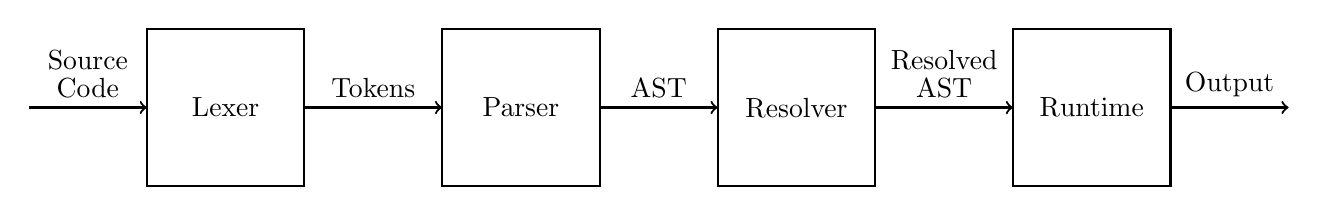
\begin{tikzpicture}
    % Draw the boxes
    \draw[thick] (-4.5, 0) rectangle (-2.5, 2);
    \draw[thick] (-0.75, 0) rectangle (1.25, 2);
    \draw[thick] (2.75, 0) rectangle (4.75, 2);
    \draw[thick] (6.50, 0) rectangle (8.50, 2);
    
    % Labels inside the boxes
    \node at (-3.5, 1) {Lexer};
    \node at (0.25, 1) {Parser};
    \node at (3.75, 1) {Resolver};
    \node at (7.5, 1) {Runtime};
    
    % Arrows and labels between boxes
    \draw[->, thick] (-2.5, 1) -- (-0.75, 1) node[midway, above] {Tokens};
    \draw[->, thick] (1.25, 1) -- (2.75, 1) node[midway, above] {AST};
    \draw[->, thick] (4.75, 1) -- (6.50, 1) node[midway, above] {\shortstack{Resolved \\ AST}};
    
    % Input and output arrows
    \draw[->, thick] (-6, 1) -- (-4.5, 1) node[midway, above] {\shortstack{Source \\ Code}};
    \draw[->, thick] (8.50, 1) -- (10, 1) node[midway, above] {Output};
  \end{tikzpicture}
  \caption{Box-Diagram representing the phases of the Bleach Interpreter.}
\end{figure}

\subsection{Lexer/Scanner}
When it comes to the lexer/scanner, it's worth remembering the reader that its goal is to transform the received source code (which is viewed by it as a large string of characters) into a sequence of tokens that will be fed to the parser of the interpreter. Such transformation performed by the lexer is known as lexical analysis.

When it comes to the possible tokens to be generated during the lexical analysis, these are the following types of tokens recognized by the lexer:

\begin{itemize}
    \item \textbf{Single-Character Tokens:}
    \begin{table}[H]
    \centering
        \begin{tabular}{|c|c|}
        \hline
        \textbf{Token Type} & \textbf{Token} \\ \hline
        LEFT\_PAREN & \texttt{(} \\ \hline
        RIGHT\_PAREN & \texttt{)} \\ \hline
        LEFT\_BRACKET & \texttt{[} \\ \hline
        RIGHT\_BRACKET & \texttt{]} \\ \hline
        LEFT\_BRACE & \texttt{\{} \\ \hline
        RIGHT\_BRACE & \texttt{\}} \\ \hline
        COMMA & \texttt{,} \\ \hline
        DOT & \texttt{.} \\ \hline
        COLON & \texttt{:} \\ \hline
        SEMICOLON & \texttt{;} \\ \hline
        QUESTION\_MARK & \texttt{?} \\ \hline
        PLUS & \texttt{+} \\ \hline
        MINUS & \texttt{-} \\ \hline
        STAR & \texttt{*} \\ \hline
        SLASH & \texttt{/} \\ \hline
        REMAINDER & \texttt{\%} \\ \hline
        BANG & \texttt{!} \\ \hline
        EQUAL & \texttt{=} \\ \hline
        GREATER & \texttt{>} \\ \hline
        LESS & \texttt{<} \\ \hline
        \end{tabular}
        \caption{Single-Character Tokens recognized by the Lexer of Bleach's Interpreter.}
    \end{table}

    \item \textbf{Double-Character Tokens:}
    \begin{table}[H]
    \centering
        \begin{tabular}{|c|c|}
        \hline
        \textbf{Token Type} & \textbf{Token} \\ \hline
        ARROW & \texttt{->} \\ \hline
        EQUAL\_EQUAL & \texttt{==} \\ \hline
        EQUAL\_EQUAL & \texttt{!=} \\ \hline
        GREATER\_EQUAL & \texttt{>=} \\ \hline
        LESS\_EQUAL & \texttt{<=} \\ \hline        
        \end{tabular}
        \caption{Double-Character Tokens recognized by the Lexer of Bleach's Interpreter.}
    \end{table}

    \item \textbf{Multi-Character Tokens:}
    \begin{table}[H]
    \centering
        \begin{tabular}{|c|c|}
        \hline
        \textbf{Token Type} & \textbf{Token} \\ \hline
        IDENTIFIER & \texttt{(a-z|A-Z|\_)(a-z|A-Z|0-9|\_)\textsuperscript{*}} \\ \hline
        NUMBER & \texttt{[0-9]\textsuperscript{+}(.[0-9]\textsuperscript{+})?} \\ \hline
        STRING & \texttt{"(any ASCII character)\textsuperscript{*}"} \\ \hline      
        \end{tabular}
        \caption{Multi-Character Tokens recognized by the Lexer of Bleach's Interpreter.}
    \end{table}

    \item \textbf{FILE\_END Token:} This token is a special one that the Bleach interpreter supports. It is responsible for signaling the end of a \texttt{.bch} file. This token has an empty string as its lexeme. Its addition will be discussed on section 4.5.
\end{itemize}

When talking about tokens, specially identifier tokens, it is important to provide the table of keywords of a programming language. In Bleach's case, this table is shown below:
\begin{table}[H]
    \centering
    \begin{tabular}{|c|c|c|}
    \hline
    \texttt{and} & \texttt{break} & \texttt{class}  \\ \hline
    \texttt{continue} & \texttt{do} & \texttt{elif}  \\ \hline
    \texttt{else} & \texttt{false} & \texttt{for}  \\ \hline
    \texttt{function} & \texttt{if} & \texttt{inherits} \\ \hline
    \texttt{lambda} & \texttt{let} & \texttt{method} \\ \hline
    \texttt{nil} & \texttt{or} & \texttt{print} \\ \hline
    \texttt{return} & \texttt{self} & \texttt{super} \\ \hline
    \texttt{true} & \texttt{while} &  \\ \hline
    \end{tabular}
    \caption{Table with all keywords available in Bleach.}
\end{table}

Regarding the implementation of the lexer itself, the road taken to achieve such goal was to build a hand-written lexer.

The implemented hand-written lexer can successfully recognize string literals and number literals. It can also ignore whitespace characters, single-line comments and multi-line comments. On top of that, the lexer is able to successfully distinguish token that share the same initial characters on their lexemes by using the concept of lookahead and "maximal munch", both previously presented. The "maximal munch" concept is also used to identify tokens that have a keyword as their lexemes from tokens that have just an identifier as their lexemes. 

Lastly, the lexer is capable of identifying invalid characters, unterminated string literals, unterminated multi-line comments and misuse of the \texttt{':'} character.

\subsection{Parser}
When it comes to the parser, it's worth remembering the reader that its goal is to transform the received sequence of tokens into an Abstract Syntax Tree (AST) that will be fed to the resolver of the interpreter. This conversion executed by the parser is known as syntax analysis.

Regarding the possible AST nodes to be generated during the syntax analysis, they can be divided into two groups of nodes (expressions and statements). These groups are structured as displayed below:

\begin{table}[h!]
\centering
    \begin{tabular}{|c|c|}
    \hline
    \textbf{Expr} & \textbf{Stmt} \\ \hline
    Assign & Block \\ \hline
    Binary & Break \\ \hline
    Call & Class \\ \hline
    Get & Continue \\ \hline
    Grouping & DoWhile \\ \hline
    LambdaFunction & Expression \\ \hline
    ListLiteral & For \\ \hline
    Literal & Function \\ \hline
    Logical & If \\ \hline
    Self & Print \\ \hline
    Set & Return \\ \hline
    Super & Var \\ \hline  
    Ternary & While \\ \hline
    Unary &  \\ \hline
    Variable &  \\ \hline
    \end{tabular}
    \label{tab:AST_nodes}  % Label for referencing the table
    \caption{All possible types of AST nodes in the Bleach programming language. \newline}
\end{table}

With respect to the parsing technique that is behind the parser component of the implemented Bleach interpreter, the chosen one was the Recursive-Descent parsing technique. With this in mind, it's important to present the BNF-grammar of Bleach: \newline

\scalebox{0.75}{
\[
\begin{array}{rcl}
\texttt{program}   & ::= & \texttt{statement\textsuperscript{*} EOF} \\[1pt]
\texttt{statement} & ::= & \texttt{block | breakStmt | classDeclStmt | continueStmt | doWhileStmt} \\
                     &     & \texttt{| exprStmt | forStmt | funcDeclStmt | ifStmt | printStmt} \\
                     &     & \texttt{| returnStmt | varStmt | whileStmt} \\[1pt]
\texttt{block} & ::= & \texttt{"\{" statement\textsuperscript{*} "\}"} \\
\texttt{breakStmt} & ::= & \texttt{"break" ";"} \\[1pt]
\texttt{classDeclStmt} & ::= & \texttt{"class" IDENTIFIER ( "inherits" IDENTIFIER )? "\{" methodDeclStmt\textsuperscript{*} "\}"} \\[1pt]
\texttt{methodDeclStmt} & ::= & \texttt{"method" method} \\[1pt]
\texttt{method} & ::= & \texttt{IDENTIFIER "(" parameters? ")" block} \\[1pt]
\texttt{continueStmt} & ::= & \texttt{"continue" ";"} \\[1pt]
\texttt{doWhileStmt} & ::= & \texttt{"do" block "while" "(" expression ")" ";"} \\[1pt]
\texttt{exprStmt} & ::= & \texttt{expression ";"} \\[1pt]
\texttt{forStmt} & ::= & \texttt{"for" "(" ( varDecl | exprStmt | ";" ) expression? ";" expression? ")" block} \\[1pt]
\texttt{funcDeclStmt} & ::= & \texttt{"function" function} \\[1pt]
\texttt{function} & ::= & \texttt{IDENTIFIER "(" parameters? ")" block} \\[1pt]
\texttt{parameters} & ::= & \texttt{IDENTIFIER ( "," IDENTIFIER )\textsuperscript{*}} \\[1pt]
\texttt{ifStmt} & ::= & \texttt{"if" "(" expression ")" statement ("elif" "(" expression ")" statement )*} \\[1pt]
\texttt{} & & \texttt{( "else" statement )? } \\[1pt]
\texttt{printStmt} & ::= & \texttt{"print" expression ";"} \\[1pt]
\texttt{returnStmt} & ::= & \texttt{"return" expression? ";"} \\[1pt]
\texttt{varDeclStmt} & ::= & \texttt{"let" IDENTIFIER ("=" expression )? ";"} \\[1pt]
\texttt{whileStmt} & ::= & \texttt{"while" "(" expression ")" block} \\[1pt]
\texttt{expression} & ::= & \texttt{assignment} \\[1pt]
\texttt{assignment} & ::= & \texttt{( call "." )? IDENTIFIER "=" assignment | ternary} \\[1pt]
\texttt{ternary} & ::= & \texttt{logic\_or ( "?" expression ":" expression )*} \\[1pt]
\texttt{logic\_or} & ::= & \texttt{logic\_and ( "or" logic\_and )*} \\[1pt]
\texttt{logic\_and} & ::= & \texttt{equality ( "and" equality )*} \\[1pt]
\texttt{equality} & ::= & \texttt{comparison ( ( "==" | "!=" ) comparison )*} \\[1pt]
\texttt{comparison} & ::= & \texttt{term ( ( ">" | ">=" | "<" | "<=" ) term )*} \\[1pt]
\texttt{term} & ::= & \texttt{factor ( ( "+" | "-" ) factor )*} \\[1pt]
\texttt{factor} & ::= & \texttt{unary ( ( "*" | "/" | "\%" ) unary )*} \\[1pt]
\texttt{unary} & ::= & \texttt{( "!" | "-" ) unary | call} \\[1pt]
\texttt{call} & ::= & \texttt{primary ( "(" arguments? ")" | "." IDENTIFIER )*} \\[1pt]
\texttt{arguments} & ::= & \texttt{expression ( "," expression )*} \\[1pt]
\texttt{primary} & ::= & \texttt{"true" | "false" | "nil" | NUMBER | STRING | IDENTIFIER | "super" "." IDENTIFIER }  \\[1pt]
\texttt{} &  & \texttt{| "(" expression ")" | "[" ( expression ( "," expression )* )? "]"} \\[1pt]
\texttt{lambdaFunctionExpr} & ::= & \texttt{"lambda" "->"  "(" parameters? ")" block} \\[1pt]
\end{array}
\]
}

In other words, the grammar of Bleach is defined by the set of rules that have been just presented. Such rules are the entities that control how expressions and statements are formed in this particular programming language.

For example, by analyzing the BNF-Grammar presented, it becomes clear to the reader the precedence of the binary arithmetical operators. The operators \texttt{"*"}, \texttt{"/"} and \texttt{"\%"} have the same precedence among them, but have more precedence when compared to the operators \texttt{"+"} and \texttt{"-"}, which also have the same precedence among them.

Going further, as mentioned previously, the parser is implemented with a top-down approach called Recursive-Descent parsing. In the case of the implemented interpreter, this parser is hand-written, since, as explained in Chapter 2, this particular parsing technique is basically a direct translation of a grammar to code that makes use of recursive functions, which makes its implementation straight-forward.

Concerning the parsing phase and the AST generation, as explained in Chapter 2, a recursive-descent parser starts the parsing process from the outermost grammar rule, which in Bleach's case is the \texttt{program} rule, and executes the process already explained when it comes to a top-down recursive descent parsing strategy.

One of the most important aspects of parsing is error reporting. In the parsing phase, the kind of error that is reported is commonly know as syntax error.

Following the guidelines presented in Chapter 2, to deal with syntax errors, the parser component of the implemented interpreter implements the ideas of "panic mode" and "error recovery". When a parser enters such mode, it needs to keep parsing process going until and continue to report more valid syntax errors until it reaches the end of the tokens sequence. To achieve this goal, the parser has a synchronization mechanism that looks for "synchronization points" from which the parser can continue the parsing process without issues. When in synchronization the parser ignores any tokens until it finds one that is a "synchronization point" and, in Bleach's case, such points are between statements.

\subsection{Resolver}
The resolver is a component of the interpreter responsible for performing a semantic analysis through the AST generated by the parser in the previous phase. To do that such traversal on the AST the Visitor design pattern is used, since it is better suited for this type of task, as explained previously in Chapter 2. 

Even though the resolver performs a semantic analysis pass over the source code, it is a simple and straight-forward one. This pass is in charge of discovering where variables were declared and guarantee that they are properly used within their scope. This component is able to resolve variable references by traversing the AST generated by the parser and associating each variable with its corresponding environment/scope inside which it was defined.

As a way to make these associations correctly the resolver has a stack of environments/scopes in which the the environment/scope at the top of the stack is the current environment/scope being analyzed. For instance, the resolver component always creates a new environment/scope and pushes it to the top of the mentioned stack every time it starts the visiting of one of the following types of AST node: \texttt{LambdaFunction}, \texttt{Block}, \texttt{Class}, \texttt{DoWhile}, \texttt{For}, \texttt{While}. When the visiting of such nodes is ended, the environment/scope at the top of the previously mentioned stack is popped and the AST traversal continues. Still on this aspect, the resolver is responsible for providing the runtime the information necessary to find the correct variable to which a certain identifier is referring to in the chain of environments created at runtime.

Diving the deeper in this respect, the resolver is also able of reporting different types of errors related to variable declaration and usage.
\begin{itemize}
    \item The resolver is able to find a variable re-declaration inside the same environment/scope and report it as an error.
    \item The resolver is also able to identify that a variable is being used in its own initializer expression and report it as an error.   
\end{itemize}

On top of that, the resolver component of the Bleach interpreter is capable of catching other errors, such as:
\begin{itemize}
    \item Usage of the \texttt{self} keyword outside of a class declaration statement.
    \item Usage of the \texttt{super} keyword outside of a class declaration statement.
    \item Usage of the \texttt{super} keyword inside a class declaration statement that is not a subclass from another class.
    \item Usage of the \texttt{break} keyword outside of any loop statement (\texttt{for}, \texttt{do-while}, \texttt{while}).
    \item Usage of the \texttt{continue} keyword outside of any loop statement (\texttt{for}, \texttt{do-while}, \texttt{while}).
    \item Usage of a class as the superclass of itself.
    \item Usage of the \texttt{return} keyword outside of a function, anonymous/lambda function or method.
    \item Usage of the \texttt{return} keyword inside the \texttt{init} method of a class declaration statement.
\end{itemize}

\subsection{Runtime}
The runtime is the last component of the interpreter. In short, this component is responsible for executing statements, evaluating expressions, performing control-flow, managing environments/scopes with their variables and respective values and also throwing runtime errors whenever required. From a different point of view, the runtime can be viewed as the engine responsible for executing code accordingly with the semantics of the implemented programming language.

As previously explained the implemented interpreter for the Bleach programming language presented in this document is a Tree-Walk one. This type of interpreter works, as earlier explained in Chapter 2, by executing a recursive traversal on the AST and performing different actions depending on the type of the AST's node that is currently being visited. All types of AST's node were also previously presented in Table~\ref{tab:AST_nodes}.

Dealing with the first group of AST nodes, the ones that represent expressions, the behavior of the runtime will fundamentally be the same: it will visit the node that represents an expression, then evaluate the expression, finally it will produce the value from said expression and will move on to continue the recursive traversal of the abstract syntax tree. 
However, the evaluation of these AST expression nodes consistently varies accordingly with the specific expression in question. A rundown of these specific behaviors regarding each type of expression node is presented beneath:
\begin{itemize}
    \item \textbf{Assign:} When visiting this kind of expression node, the interpreter first evaluates the RHS (right-hand side) of this expression node. This evaluation will produce a value that must be assigned to the LHS (left-hand side) of this very same node. However, the evaluation of the LHS is a bit different than the one made with respect to the RHS. This one evaluates to a location in-memory in which the value obtained through the evaluation of the RHS will be stored. In order to find out the correct memory location, the runtime makes use of information previously computed by the resolver about variable resolution and environments. By default, this visiting returns the value from the RHS evaluation.
    \item \textbf{Binary:} When visiting this type of expression node, the interpreter first evaluates its left operand and, then, the right one. Finally, it performs the operation depending on the type of operator that this node stores and returns the result of such operation.
    \item \textbf{Call:} When visiting this sort of expression node, the interpreter first evaluates the callee of this node in order to figure out if it is a valid one (a function, an anonymous/function, a native function, a method, a class, or a method from the \texttt{list} and \texttt{str} built-in types). Once this is done, the interpreter evaluates each of the expressions that represent the arguments of the call and store such values appropriately. Finally, it makes the call to the callee passing the evaluated arguments. This sort of expression node returns the same thing the function that has been called returns.
    \item \textbf{Get:} When visiting this kind of expression node, the interpreter first evaluates the expression representing the entity on which the property is trying to be accessed. If such expression evaluates to an instance of a class, a value of type \texttt{list} or a value of type \texttt{str}, then the interpreter tries to find the value associated to the property and, finally, returns it.
    \item \textbf{Grouping:} When visiting this type of expression node, the interpreter just evaluates and, ultimately, returns the produced value by the nested expression within this type of node, since a Grouping node essentially represents a pair of parentheses.
    \item \textbf{LambdaFunction:} When visiting this kind of expression node, the interpreter just creates a runtime representation of the anonymous/lambda function by using the visited expression itself along with the current environment/scope that is in, since it will serve as the closure of such anonymous function.
    \item \textbf{ListLiteral:} When visiting this sort of expression node, the interpreter creates the runtime representation of a list. Then it evaluates each expression present inside the ListLiteral expression and appends the result to the runtime portrayal of the mentioned list. In the end, it returns such list.
    \item \textbf{Literal:} When visiting this type of expression node, the interpreter just evaluates the value associated with the literal and returns it.
    \item \textbf{Logical:} This expression node is a basically a specialization of the "Binary" node because it can only perform the following operations: \texttt{and}, \texttt{or}. Still, it evaluates the left operand first and, according to the left value and the operator itself, tries to perform a short-circuiting. If that's not possible, it evaluates the right operand, produces the corresponding value by following the rules of Boolean Algebra and, finally, returns the produced value.
    \item \textbf{Self:} When visiting this kind of expression node, the interpreter uses it and the token that represents that particular \texttt{self} keyword to figure out at which environment the required variable is at (remember that the \texttt{self} is a name that references the current instance of a class, making it, in practice a variable). Once at such environment, the interpreter returns the instance bound to such name.
    \item \textbf{Set:} The visiting process of this expression node is very similar to that of the "Get" node. In this particular expression node, the interpreter first evaluates the expression representing the value that works as the RHS. Then, the interpreter evaluates the expression that represents the entity that contains the attribute that is about to receive the generated RHS value. If the evaluation of the expression that represents an entity results in a valid value (an instance of a class), then the interpreter searches for the attribute inside such value (which will result in a LHS value) in order to perform the binding between them. Finally, this visiting process returns the RHS value.
    \item \textbf{Super:} When visiting this sort of expression node, the interpreter first retrieves the superclass of the class whose "Super" node is being currently visited. Once this is finished, the interpreter then retrieves the instance of the class whose "Super" node is being visited. Finally, the interpreter searches and returns the superclass version of the method required in the "Super" expression node.    
    \item \textbf{Ternary:} When visiting this particular expression node, the interpreter first evaluates its first operand, known as condition. If the result produced by such evaluation is \texttt{true}, then the ternary operator evaluates and returns its second operand, the one between \texttt{"?"} and \texttt{":"}. Otherwise, this operator evaluates and returns its third operand, the one that appears after \texttt{":"}.
    \item \textbf{Unary:} When visiting this type of expression node, the interpreter first evaluates its unique operand, commonly known as right operand. After this, it performs the operation, given the operator, on the operand, produces and, at last, returns the corresponding value.
    \item \textbf{Variable:} When visiting this type of expression node, the interpreter uses the expression node itself, which represents a variable usage, combined with the variable's token to figure out at which environment the required variable is at. Then, the runtime accesses that environment, retrieves and returns the value associated to the required variable. 
\end{itemize}

Now analyzing the second group of AST nodes, the one that contains nodes representing different kinds of statement, which can be called statement nodes:
\begin{itemize}
    \item \textbf{Block:} When visiting this kind of statement node, the interpreter first stores the current environment (the implementation of the concept of lexical scope). Then, sets the current environment of the interpreter to another that has been created and whose enclosing one is the one that has been on use before the interpreter started the visit to this statement node. On this new environment current environment, the interpreter executes the statements present in the "Block" node one-by-one from top to bottom. After finishing this, it restore the environments to the initial configuration before starting the visit of this type of statement node.
    \item \textbf{Break:} When visiting this sort of statement node, the interpreter just throws an instance of a "Break" entity that will be caught by the runtime when visiting any loop statement node (\texttt{do-while}, \texttt{for}, \texttt{while}) and dealt with by it. This entity is responsible for simulating the behavior of loop interruption at runtime caused by the use of a \texttt{break} statement.
    
    \item \textbf{Class:} When visiting this type of statement node, the interpreter first checks whether the node has an expression that might evaluate to a superclass. If that's the case, such expression is properly evaluated and its result is stored for later use. After this, the interpreter creates a binding at the current environment it is in between the class name and the \texttt{nil} value. If the "Class" statement node indeed has a superclass associated to it, a nesting environment is created and a binding between the name \texttt{super} and the runtime representation of the superclass is generated. Then, for each method declared inside this statement node, its respective runtime representation is generated and stored inside the runtime representation of the class in a way that associates the name of the method and its respective runtime depiction. At last, the runtime portrayal of the class is populated with the needed information.
    
    \item \textbf{Continue:} When visiting this kind of statement node, the interpreter just throws an instance of a "Continue" entity that will be caught by the runtime when visiting any loop statement node (\texttt{do-while}, \texttt{for}, \texttt{while}) and dealt with by it. This entity is responsible for simulating the behavior of interrupting an iteration of a loop and going to the next iteration by the use of a \texttt{continue} statement.
    \item \textbf{DoWhile:} When visiting this sort
    
    \item \textbf{Expression:} When visiting this type
    
    \item \textbf{For:} When visiting this kind 
    
    \item \textbf{Function:} When visiting this sort
    
    \item \textbf{If:} When visiting this type
    
    \item \textbf{Print:} When visiting this kind
    
    \item \textbf{Return:} When visiting this sort
    
    \item \textbf{Var:} When visiting this type
    
    \item \textbf{While:} When visiting this kind

\end{itemize}

\section{Challenges, Decisions and Trade-Offs}
upeaaa 
\textbf{Em Lexer: Falar sobre a decisão de escolher um hand-written lexer, comparar com outras opções. Desafios para lidar com o reconhecimento de strings, identificadores, numeros, comentários, "maximal munch" theorem, e suporte à funções nativas (uso de ':').}

\textbf{Falar sobre implementação de funções nativas: permissão do uso do caracter ':' em certos casos (restritos pelo Lexer.hpp e pelo Parser.hpp). Falar sobre a implementação das funções nativas em si dentro do arquivo "NativeFunctions.hpp'. Falar sobre o binding feito em escopo global do interpretador para permitir o acesso às funções nativas e no método VisitCallExpr do arquivo 'Interpreter.hpp'.}

\textbf{Em Parser: Falar sobre a decisão de escolher um hand-written parser que segue a abordagem top-down recursive.}

\textbf{Falar sobre a decisão de permitir a redeclaração de variáveis globais em Bleach e o porquê disso.}

\textbf{Falar sobre a decisão de implementar single-inheritance ao invés de multiple-inheritance. Isso pode entrar tanto como "Future Work" como ser um assignment para uma turma.}

\textbf{Falar sobre a decisão de usar um Handwritten Lexer/Scanner.}

\textbf{Falar sobre a decisão de usar Recursive-Descent Parsing.}

\textbf{Falar sobre a decisão de usar um Tree-Walk Interpreter ao invés de uma ByteCode VM ou de um Compilador.}


\section{What Makes Bleach Shine and How It Can Be Used In a Classroom Environment}
